%% This is file `elsarticle-template-1-num.tex',
%%
%% Copyright 2009 Elsevier Ltd
%%
%% This file is part of the 'Elsarticle Bundle'.
%% ---------------------------------------------
%%
%% It may be distributed under the conditions of the LaTeX Project Public
%% License, either version 1.2 of this license or (at your option) any
%% later version.  The latest version of this license is in
%%    http://www.latex-project.org/lppl.txt
%% and version 1.2 or later is part of all distributions of LaTeX
%% version 1999/12/01 or later.
%%
%% Template article for Elsevier's document class `elsarticle'
%% with numbered style bibliographic references
%%
%% $Id: elsarticle-template-1-num.tex 149 2009-10-08 05:01:15Z rishi $
%% $URL: http://lenova.river-valley.com/svn/elsbst/trunk/elsarticle-template-1-num.tex $
%%
\documentclass[preprint,12pt]{elsarticle}
\usepackage[options ]{algorithm2e}

\usepackage{graphicx}

%% Use the option review to obtain double line spacing
%% \documentclass[preprint,review,12pt]{elsarticle}

%% Use the options 1p,twocolumn; 3p; 3p,twocolumn; 5p; or 5p,twocolumn
%% for a journal layout:
%% \documentclass[final,1p,times]{elsarticle}
%% \documentclass[final,1p,times,twocolumn]{elsarticle}
%% \documentclass[final,3p,times]{elsarticle}
%% \documentclass[final,3p,times,twocolumn]{elsarticle}
%% \documentclass[final,5p,times]{elsarticle}
%% \documentclass[final,5p,times,twocolumn]{elsarticle}

%% The graphicx package provides the includegraphics command.
\usepackage{graphicx}
%% The amssymb package provides various useful mathematical symbols
\usepackage{amssymb}
%% The amsthm package provides extended theorem environments
%% \usepackage{amsthm}

%% The lineno packages adds line numbers. Start line numbering with
%% \begin{linenumbers}, end it with \end{linenumbers}. Or switch it on
%% for the whole article with \linenumbers after \end{frontmatter}.
\usepackage{lineno}

%% natbib.sty is loaded by default. However, natbib options can be
%% provided with \biboptions{...} command. Following options are
%% valid:

%%   round  -  round parentheses are used (default)
%%   square -  square brackets are used   [option]
%%   curly  -  curly braces are used      {option}
%%   angle  -  angle brackets are used    <option>
%%   semicolon  -  multiple citations separated by semi-colon
%%   colon  - same as semicolon, an earlier confusion
%%   comma  -  separated by comma
%%   numbers-  selects numerical citations
%%   super  -  numerical citations as superscripts
%%   sort   -  sorts multiple citations according to order in ref. list
%%   sort&compress   -  like sort, but also compresses numerical citations
%%   compress - compresses without sorting
%%
%% \biboptions{comma,round}

% \biboptions{}

\journal{Journal Name}

\begin{document}


\begin{frontmatter}

%% Title, authors and addresses

\title{Measuring the Efficiency of Canadian Healthcare at the Provincial Level}
%% use the tnoteref command within \title for footnotes;
%% use the tnotetext command for the associated footnote;
%% use the fnref command within \author or \address for footnotes;
%% use the fntext command for the associated footnote;
%% use the corref command within \author for corresponding author footnotes;
%% use the cortext command for the associated footnote;
%% use the ead command for the email address,
%% and the form \ead[url] for the home page:
%%
%% \title{Title\tnoteref{label1}}
%% \tnotetext[label1]{}
%% \author{Name\corref{cor1}\fnref{label2}}
%% \ead{email address}
%% \ead[url]{home page}
%% \fntext[label2]{}
%% \cortext[cor1]{}
%% \address{Address\fnref{label3}}
%% \fntext[label3]{}


%% use optional labels to link authors explicitly to addresses:
%% \author[label1,label2]{<author name>}
%% \address[label1]{<address>}
%% \address[label2]{<address>}

\author{Bassim Eledath}
\author{Abhishek Sharma}
\author{Assel Ismoldayeva}
\author{Yuqi Zhang}
\address{San Francisco, California}

\begin{abstract}
%% Text of abstract
American politicians often cite Canada's single-payer as a positive example when criticizing the lack of healthcare reform in the United States. However, an internal complaint of Canadian citizens regards the drastic wait times that precede important medical operations. After hearing conflicting opinions on the efficiency of Canada's healthcare system, we posed the following questions:
\\ \\ 
\textbf{Can we develop a quantitative rank based method to evaluate system efficiency at the Provincial Level? Can this rank be based on indicators that measure health care outcomes such as lifetime expectancy and wait times? Given this information, can we evaluate "similar" provinces to establish ceteris paribus (all else equal) relationships between expenditure and health care efficiency?}
 


\begin{center}
    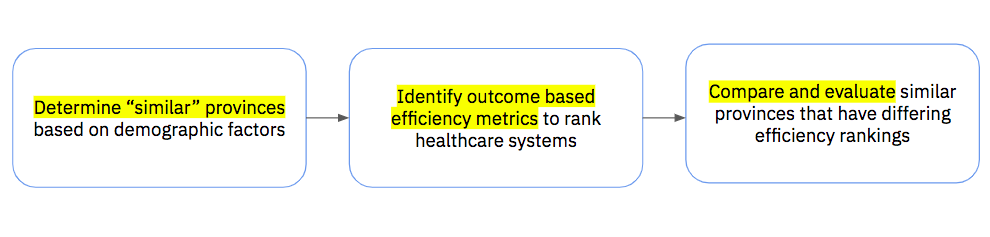
\includegraphics[scale=0.4]{images/screenshot.png}
\end{center} 

This is the question that our team set out to answer. Our workflow consisted of the following steps:
			
\begin{enumerate}
	\item Determine Similar Provinces: We use features such as proportional of aborginal population, population density etc. to find provinces that are similar to each other. We use k-means to cluster these provinces.
    \item Determine Relevant Outcome Based metrics to Rank Provinces on health care efficiency: We use healthcare outcome indicators such as lifetime expectancy and wait time to rank provinces based on efficiency.
    \item Compare and Contrast “similar” provinces with differing efficiency scores: We find similar provinces that vary greatly in terms of our efficiency rank to evaluate why this discrepancy arises based on expenditure data.
\end{enumerate}

By building an efficiency metric based on infant mortality, life expectancy at birth, live expectancy at age 65, and wait times, we are able to compare each province in Canada from most efficient to least. We then use this metric to compare two Provinces (Alberta and British Columbia) that are similar based on demographic features. These provinces are different in terms of efficiency scores, so understanding how healthcare expenditure relates to this discrepancy.

\end{abstract}



\end{frontmatter}

%%
%% Start line numbering here if you want
%%

%% main text


\newpage
\section{Technical Exposition}
\label{S:2}

\subsection{Summary of the Approach}
We have selected similar provinces to compare the efficiency of their health care systems. We have used the following criteria in our analysis:

\subsubsection{Determining Outcome Based Efficiency metrics to evaluate healthcare systems:}

\begin{itemize}
    \item Infant Mortality Rate: The number of deaths of children under one year of age per 1000 live births.
    \item Life Expectancy at Birth: The average time a newborn is expected to live, based on the year of their birth.
    \item Life Expectancy at Age 65: The average number of years that a person of age 65 can be expected to live, assuming that age-specific mortality levels remain constant. 
    \item Wait Time: The time a patient has to wait from a referral by a general practitioner to consultation with a specialist.
\end{itemize}


\subsubsection{Similarity Scoring based on the following features:}
\begin{itemize}
    \item Population count
    \item Population density
    \item Median age
    \item Percentage of population older than 65 years
    \item Unemployment rate
\end{itemize}

\begin{center}
    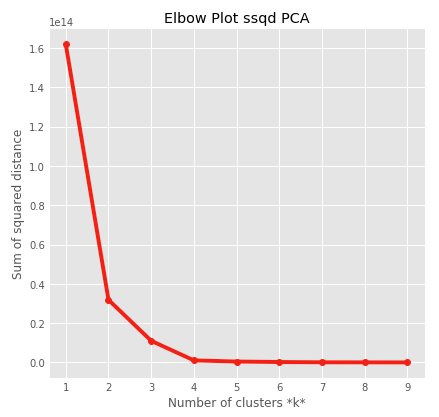
\includegraphics[scale=0.35]{elbow.png}
\end{center}
The elbow plot shows the optimal number of kmeans clusters is 4, showing 4 similar groupings of provinces.

\subsection{Initial Exploration}

When analyzing the healthcare expenditures of each province in Canada, we found some high-variance features which we decided to explore visually.

\begin{center}
    \caption{Healthcare Expenditure in Canadian Dollars over Time}
    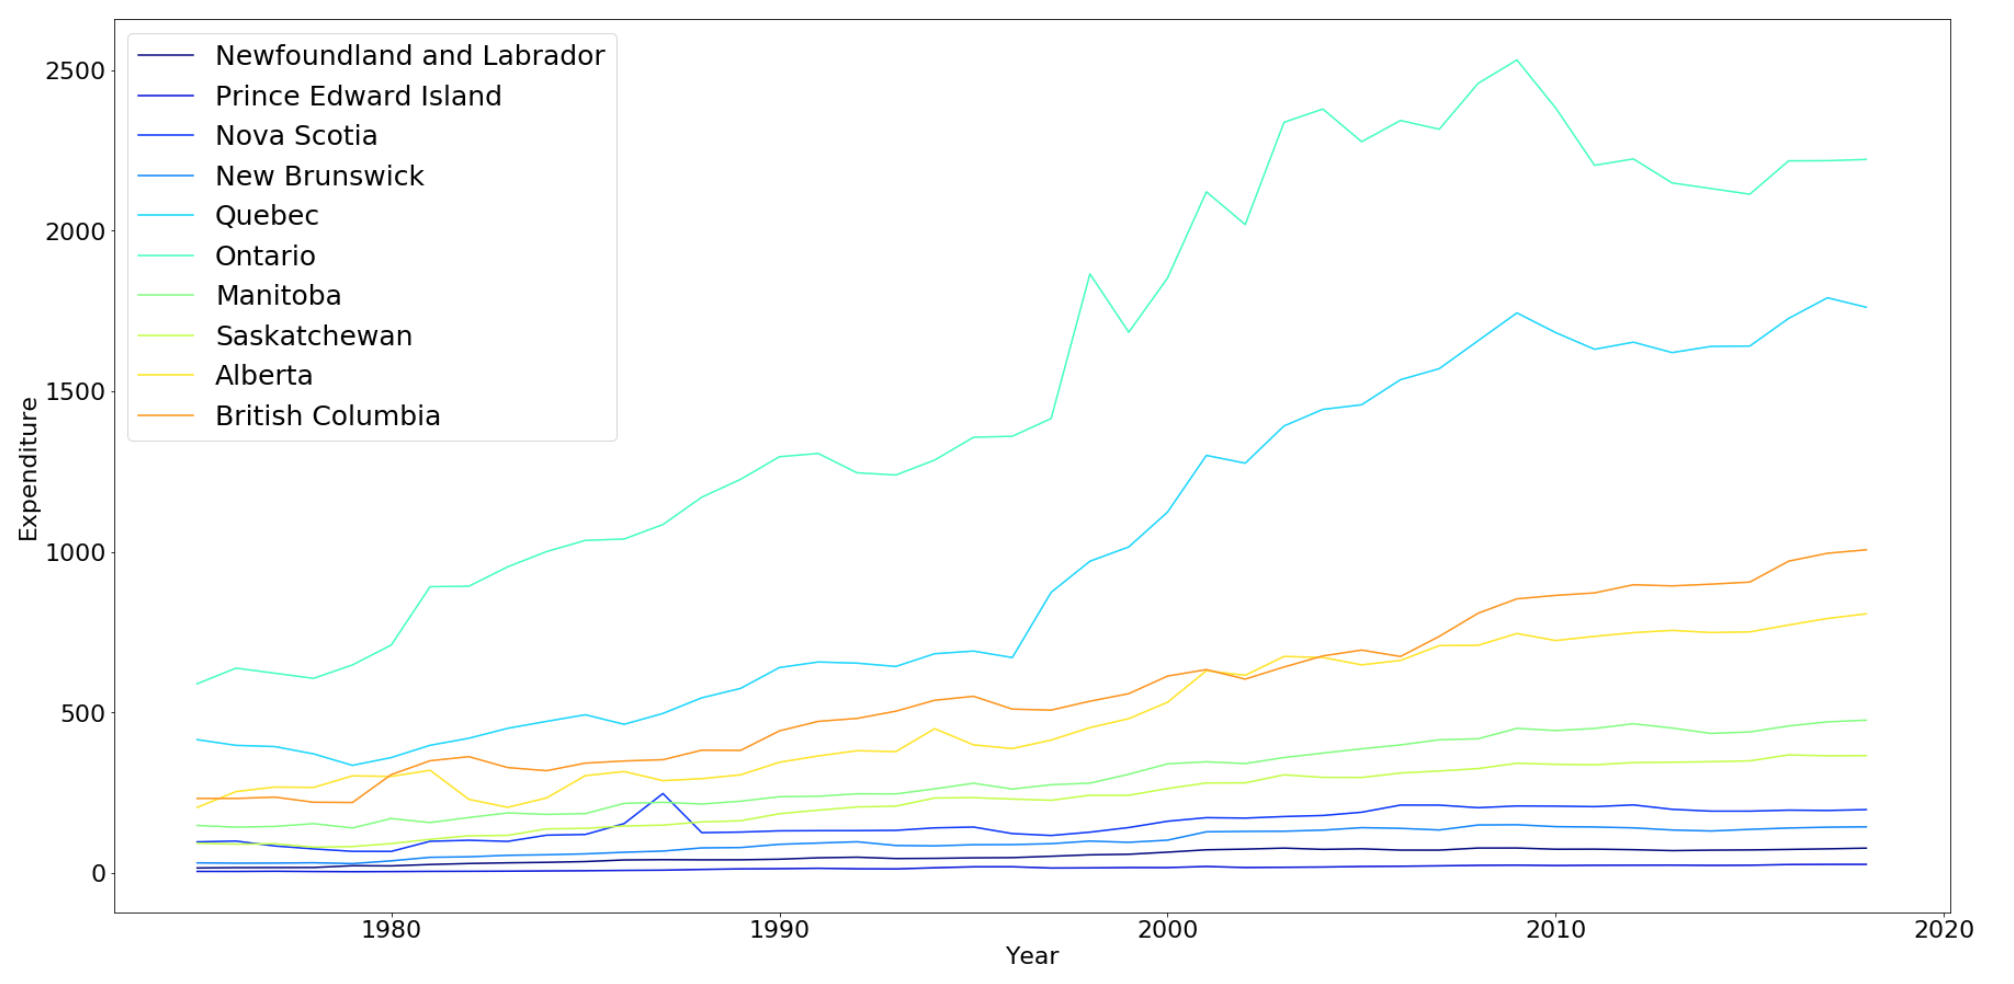
\includegraphics[scale=0.35]{images/expenditure_time.png}
\end{center}

This plot shows how some provinces chose to drastically increase healthcare spending, while others flatlined over the past few decades. 

We also noticed that the expenditure on drugs varied from province to province, as this normalized geospatial chart shows.
\begin{center}
    
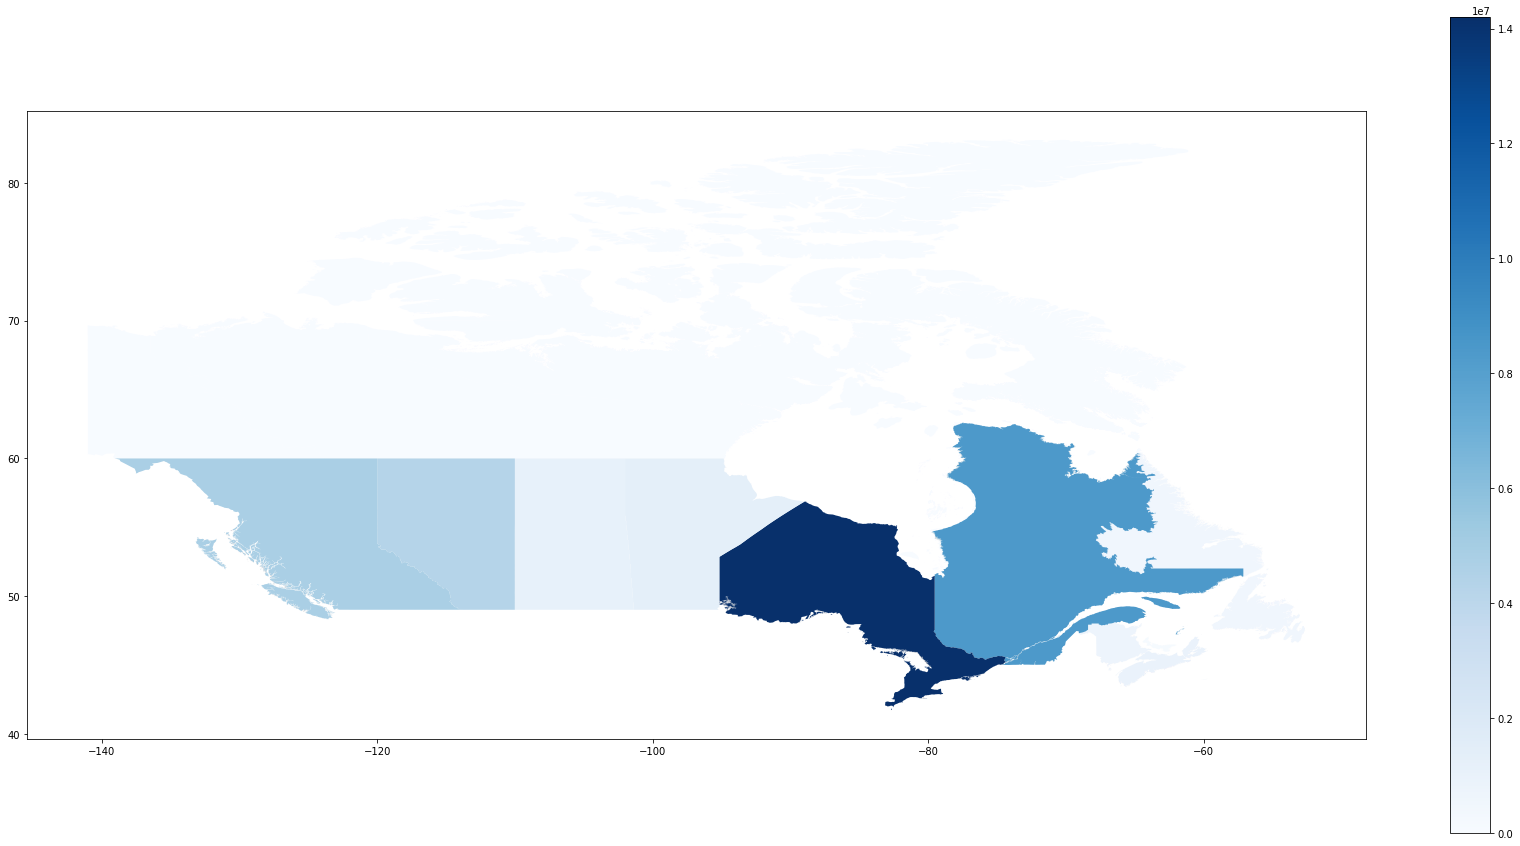
\includegraphics[scale=0.17]{images/Population_map.png}

\end{center}


\subsection{Computing Rankings}
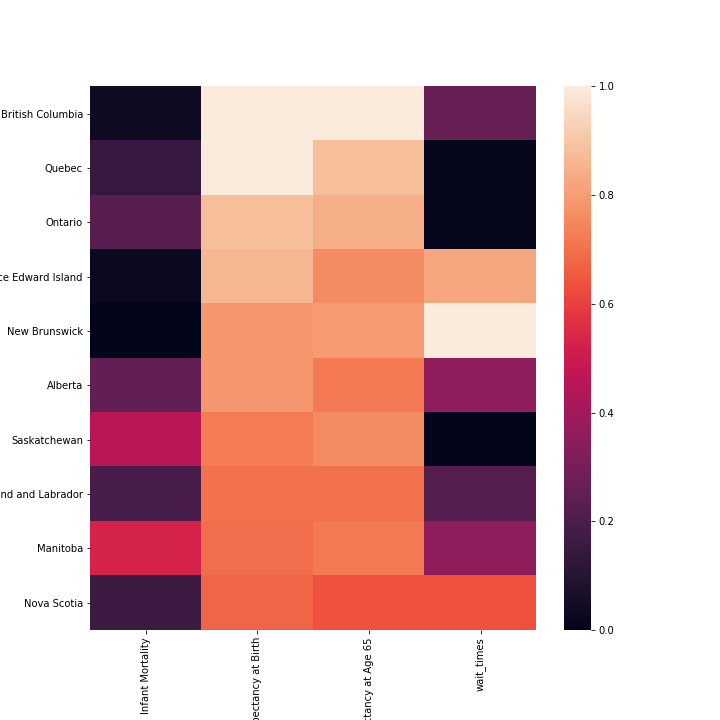
\includegraphics[scale=0.5]{heatmap_rank.png}

Our first proposition was to utilize a supervised learning algorithm to optimize weights for each feature, resulting in a comparable metric that we could use to rank the provinces. However, there is no ground-truth dataset of provincial rankings. Therefore, our algorithm would have nothing to optimize against. 

Instead, we opted to rank the features themselves by highest to lowest priority, and devised the following ranking algorithm

\\
\begin{algorithm}[H]
\SetAlgoLined
\KwResult{A ranked set of Canadian provinces}
 featuresList = [f1, f2, .. fn]; \# sorted by priority

 result = [1, 1, .. 1]; \# initialize with a 10-way tie
 
 \While{our result has any ties}{
    f = first feature from featuresList;
    
    rank tied provinces by f;
    
    remove f from featuresList;
 }
 \caption{Canadian Provincial Healthcare Ranking Algorithm}
\end{algorithm}
\\ \\
Here's how our algorithm stacks up against publicly released rankings by two Canadian think tanks. As you can see, we performed relatively well against the Conference Board of Canada, but quite poorly against the Frontier Centre for Public Policy. This is most likely because the FCPP factors in cost as a major factor for their ranking.

\begin{table}[h]
\centering
\begin{tabular}{l l l}
\hline
\textbf{Ranking} & \textbf{Spearman Rank Correlation}\\
\hline
Conference Board of Canada & 0.867 \\
Frontier Centre for Public Policy & 0.382 \\
\hline
\end{tabular}
\caption{Rank quality of our metric as compared to 2 Canadian think tanks}
\end{table}

Lastly, let's see how our rankings vary when we choose to construct them by prioritizing different features.
\begin{center}
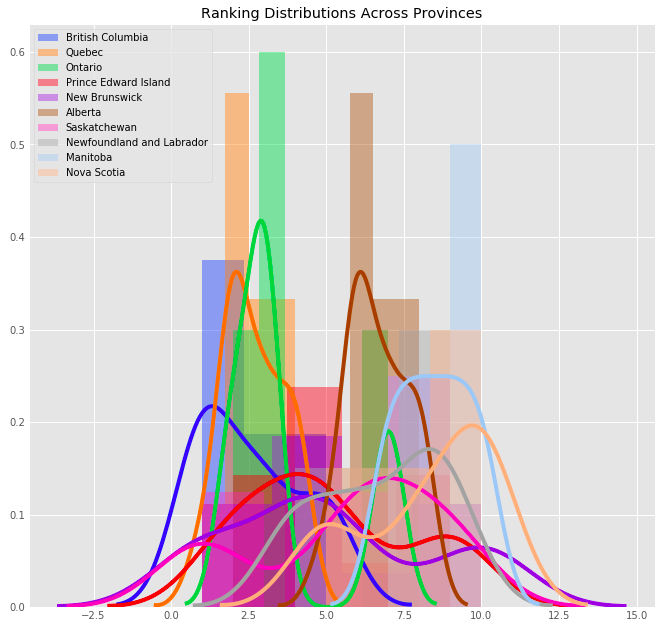
\includegraphics[scale=0.3]{images/rankdistributions.png}
\end{center}


\subsection{Comparison between Albert and British Columbia}
The previous sections show that Albert and British Columbia has very different efficiency in health care system based on our evaluation metric, however, they are considered similar provinces based on our clustering. So we take a close look at how these two provinces are different from each other.\\
\begin{center}
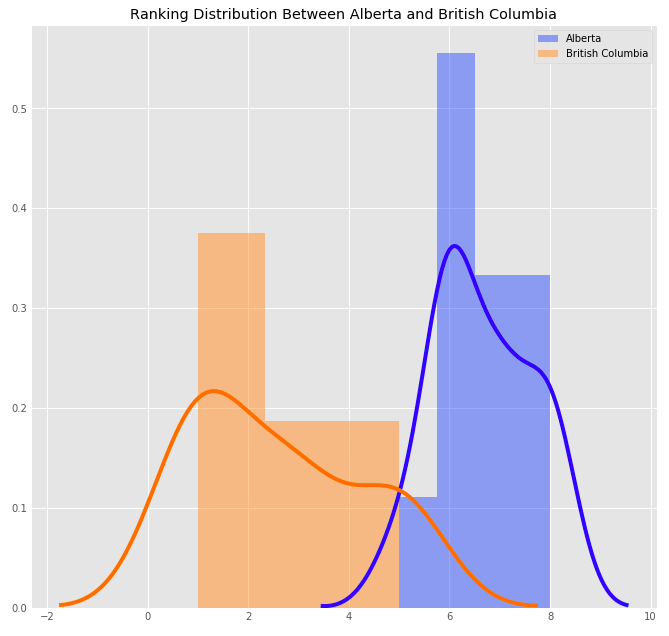
\includegraphics[scale=0.3]{images/albertabccompare.png}
\end{center}
The following two factors are the most significant after we evaluating the first 3 data sets:
\begin{enumerate}
	\item Difference in expenditure on drugs per capita by Type by source of finance in dollars of Albert and British Columbia from 1985 to 2018
	
	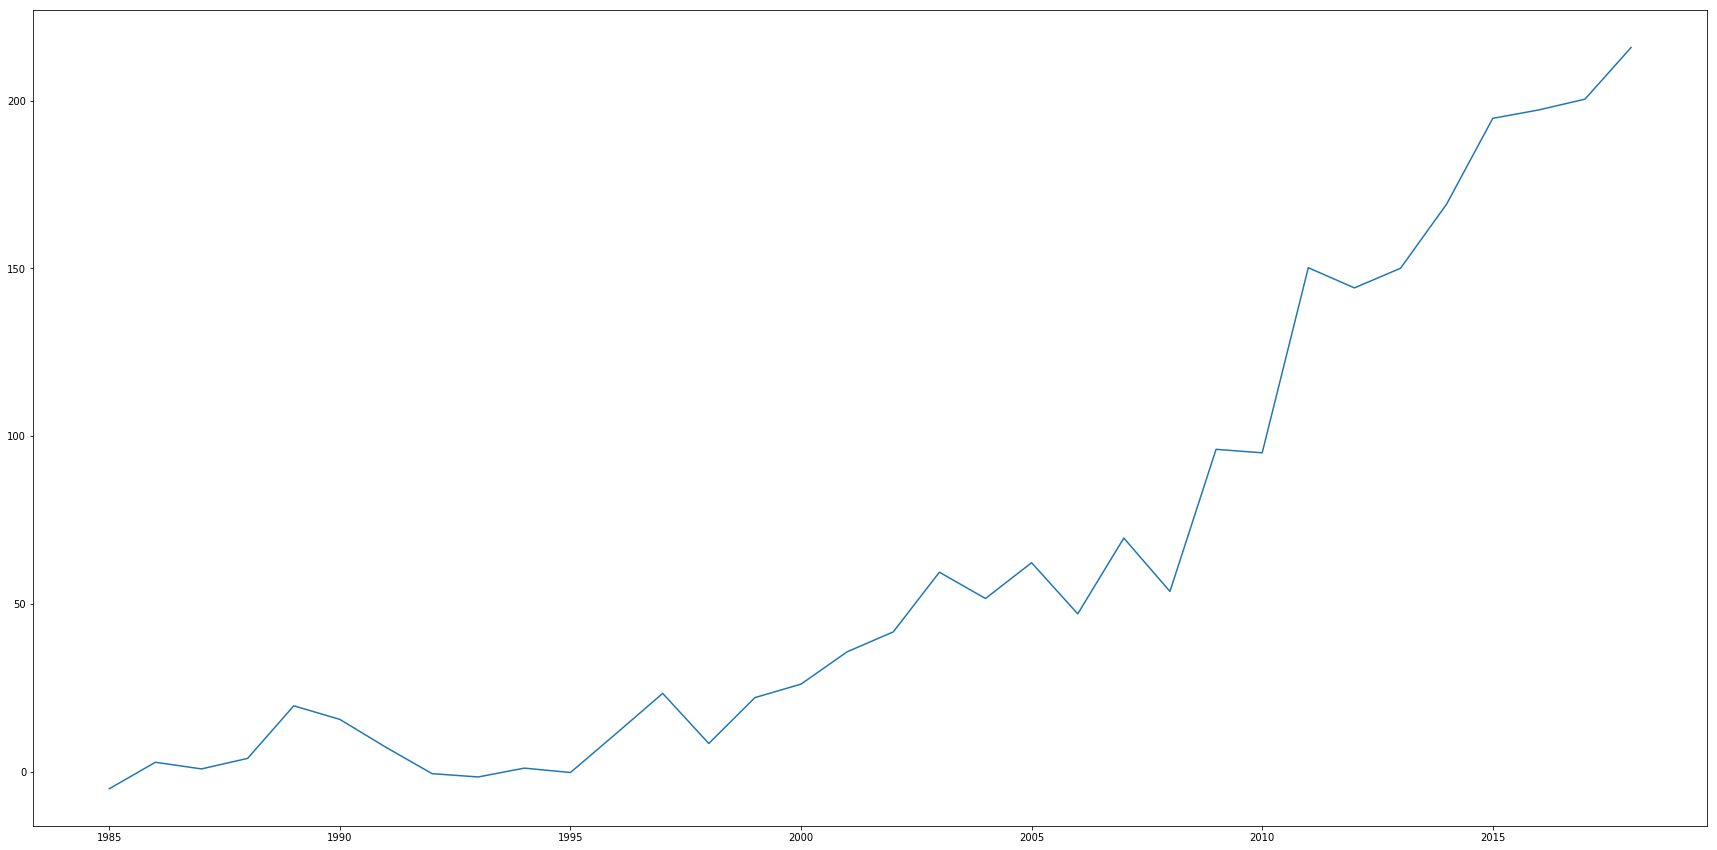
\includegraphics[scale=0.2]{images/drugdrug.png}
	
	The difference of average types of individual drugs use keeps rising since 1995 and it rises to 200 at 2018 which is around $20 \%$ considering the maximum number of types of drugs.
	
    \item Difference in Municipal government health expenditure by province/territory and Canada of Albert and British Columbia from 1985 to 2018
    
    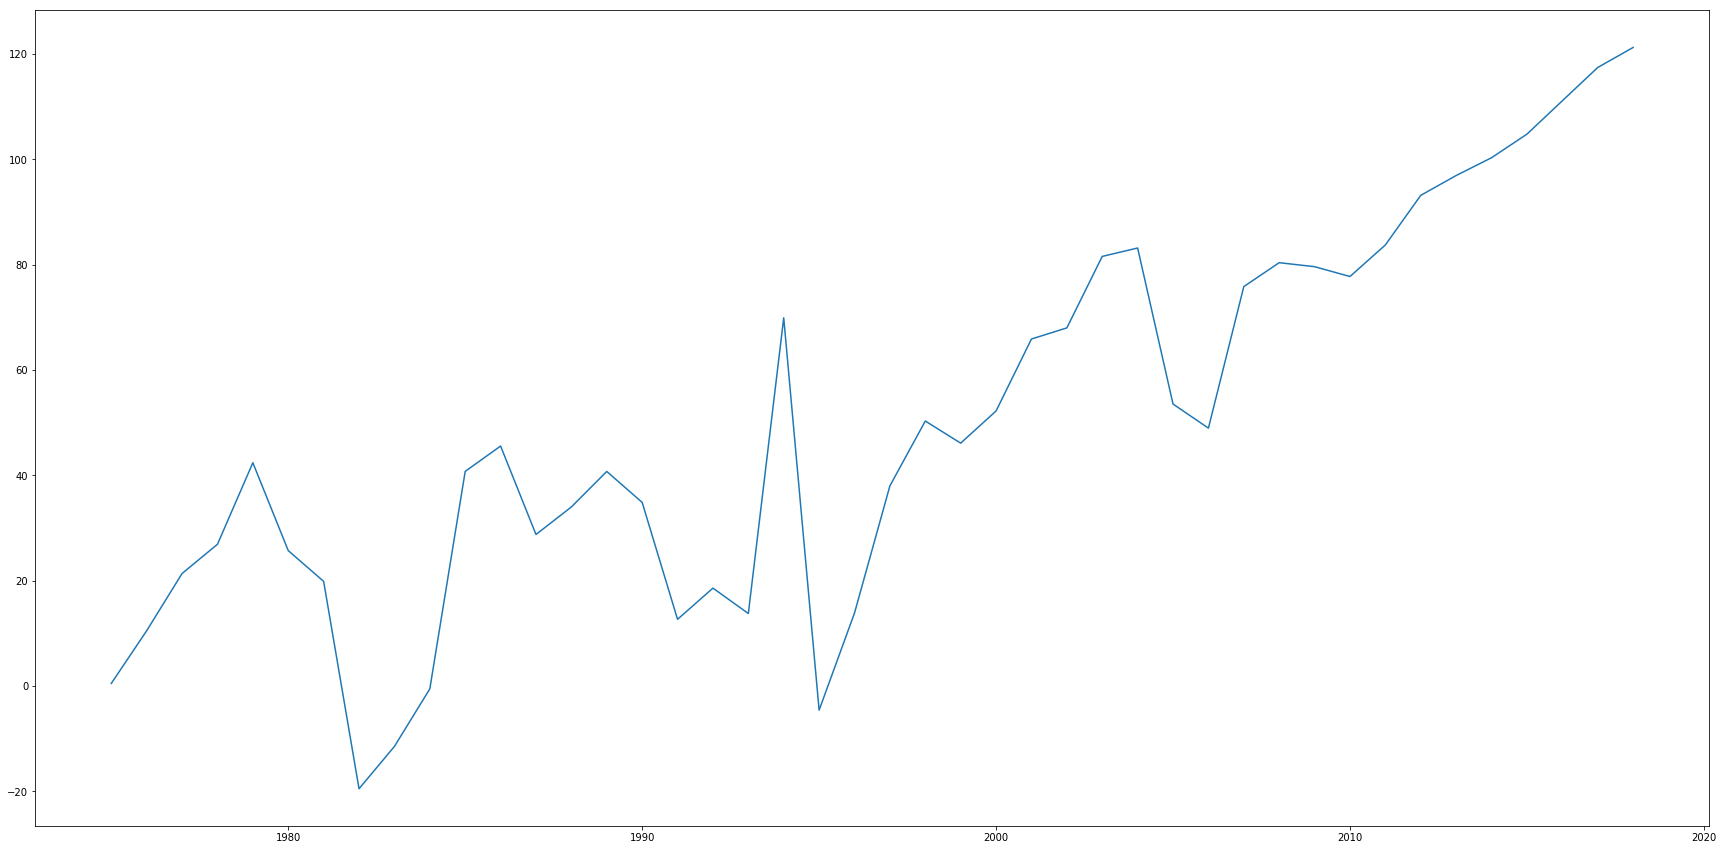
\includegraphics[scale=0.2]{download.png}
    
    The difference in municipal government health expenditure starts rising since 1995 and rises to around $50\%$ of the maximum value.
\end{enumerate}

Both graphs show the significant difference between two provinces that cause the difference in efficiency.

\newpage
\subsection{Conclusion}

Through our analysis, we were able to find a reliable source of ranking the provinces of Canada by how efficient their healthcare systems are. 

There were two provinces with similar features, Alberta and British Columbia, that had vastly different healthcare efficiencies. Upon further analysis, we deduced that these differences are due to differences in drug expenditure over the past 40 years. 

For future work, we would investigate the error rate between our ranking and that of the Frontier Centre for Public policy. 

\begin{center}
    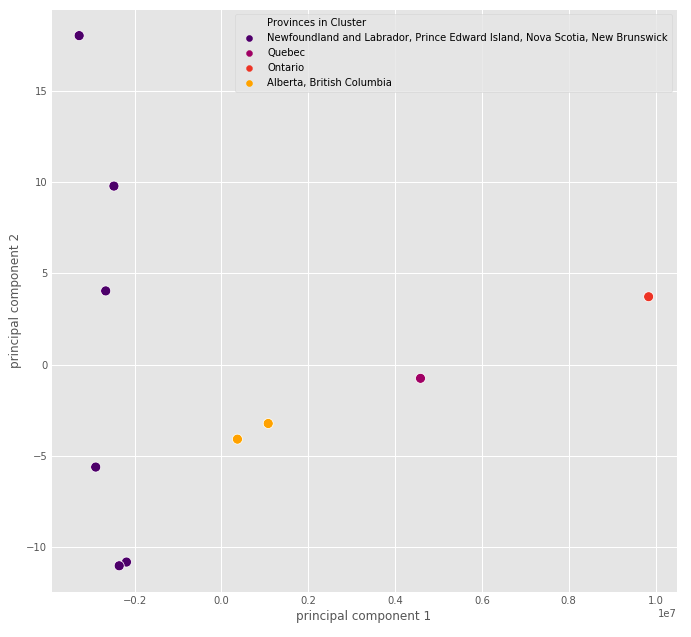
\includegraphics[scale=0.4]{images/clusters.png}
\end{center}



%% The Appendices part is started with the command \appendix;
%% appendix sections are then done as normal sections
%% \appendix

%% \section{}
%% \label{}

%% References
%%
%% Following citation commands can be used in the body text:
%% Usage of \cite is as follows:
%%   \cite{key}          ==>>  [#]
%%   \cite[chap. 2]{key} ==>>  [#, chap. 2]
%%   \citet{key}         ==>>  Author [#]

%% References with bibTeX database:



%% Authors are advised to submit their bibtex database files. They are
%% requested to list a bibtex style file in the manuscript if they do
%% not want to use model1-num-names.bst.

%% References without bibTeX database:

% \begin{thebibliography}{00}

%% \bibitem must have the following form:
%%   \bibitem{key}...
%%

% \bibitem{}

% \end{thebibliography}


\end{document}

%%
%% End of file `elsarticle-template-1-num.tex'.